\documentclass[tikz,border=1pt]{standalone}
\usepackage[T1]{fontenc}
\usepackage[utf8]{inputenc}
\usepackage{amsmath}
\usepackage{tikz}
\usetikzlibrary{calc}
\usepackage{pgfplots}
\usepgfplotslibrary{fillbetween,groupplots}

\definecolor{simColor}{HTML}{D55E00}

\pgfplotsset{
  compat=1.18,
  legend image code/.code={
    \draw[mark repeat=2,mark phase=2]
    plot coordinates {(0cm,0cm)(0.2cm,0cm)(0.4cm,0cm)};
  },
}

\begin{document}
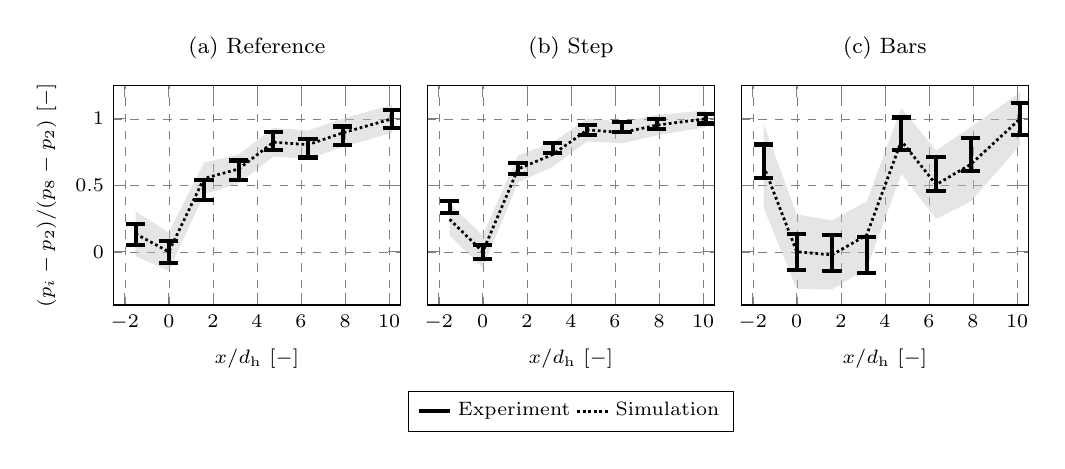
\begin{tikzpicture}

\begin{groupplot}[
  group style={
    group size=3 by 1,
    horizontal sep=0.35cm,
  },
  width=0.30\textwidth,
  height=0.23\textwidth,
  scale only axis,
  xmin=-2.5, xmax=10.5,
  ymin=-0.40, ymax=1.25,
  xtick distance=2,
  grid=major,
  grid style={line width=0.05pt, draw=gray, dashed},
  xlabel={$x/d_{\mathrm{h}}\ [-]$},
  label style={font=\fontsize{7.5pt}{12pt}\selectfont},
  tick label style={font=\fontsize{7pt}{12pt}\selectfont},
  title style={font=\fontsize{8pt}{12pt}\selectfont},
  % legend style={
  %   draw=black,
  %   fill=white,
  %   fill opacity=0.8,
  %   text opacity=1,
  %   font=\small,
  %   legend columns=3,
  %   legend cell align=center,
  % },
]

\nextgroupplot[
  title={(a) Reference},
  ylabel={$(p_i-p_2)/(p_8-p_2)\ [-]$},
  % ylabel={$p_\mathrm{rel}^+\ [-]$},
  legend to name=pressureLegend,
  legend style={
    % at={(0.95,-0.05)}, anchor=south east,
    draw=black,
    fill=white,
    fill opacity=0.8,
    text opacity=1,
    font=\fontsize{7pt}{12pt}\selectfont,
    legend columns=3,
    legend cell align=left,
    },
]
% copy reference experimental, simulation and band plots here
%% --- Experimental error bars (no centre marker) ----------------------------
\addplot[
  black, draw=none, mark=none, forget plot,
  error bars/.cd,
  y dir=both, y explicit,
  error bar style={black, solid, line width=1.5pt},
  error mark options={black, mark size=3.5pt, line width=1.5pt, rotate=90},
  error mark=-,
] coordinates {
  (-1.50341, 0.1294) +- (0, 0.0796)
  ( 0.00000, 0.0000) +- (0, 0.0815)
  ( 1.59886, 0.4654) +- (0, 0.0747)
  ( 3.17386, 0.6136) +- (0, 0.0726)
  ( 4.74886, 0.8323) +- (0, 0.0694)
  ( 6.32386, 0.7788) +- (0, 0.0702)
  ( 7.89886, 0.8727) +- (0, 0.0688)
  (10.14205, 1.0000) +- (0, 0.0670)
};
\addlegendimage{black, solid, line width=1.5pt}
% \addlegendentry{Exp. $\pm$1.45\%}
\addlegendentry{Experiment}

%% --- Simulation mean line ---------------------------------------------------
% \definecolor{simColor}{HTML}{009E73} % Okabe-Ito green — reference case
\addplot[
  black, densely dotted, mark=none, mark size=2.5pt,
  mark options={solid}, line width=1.0pt,
] coordinates {
  (-1.50341, 0.1350) ( 0.00000, 0.0000) ( 1.59886, 0.5508)
  ( 3.17386, 0.6223) ( 4.74886, 0.8234) ( 6.32386, 0.8046)
  ( 7.89886, 0.8938) (10.14205, 1.0000)
};
\addlegendentry{Simulation}

%% --- Simulation std-deviation band -----------------------------------------
\addplot[draw=none, name path=refUpper, forget plot] coordinates {
  (-1.50341, 0.3028) ( 0.00000, 0.1447) ( 1.59886, 0.6692)
  ( 3.17386, 0.7309) ( 4.74886, 0.9310) ( 6.32386, 0.9115)
  ( 7.89886, 1.0015) (10.14205, 1.1034)
};
\addplot[draw=none, name path=refLower, forget plot] coordinates {
  (-1.50341,-0.0327) ( 0.00000,-0.1447) ( 1.59886, 0.4325)
  ( 3.17386, 0.5137) ( 4.74886, 0.7158) ( 6.32386, 0.6976)
  ( 7.89886, 0.7861) (10.14205, 0.8966)
};
\addplot[gray!50, draw=none, fill opacity=0.40]
  fill between[of=refUpper and refLower];
% \addlegendentry{Sim.\ $\pm\sigma$}

\nextgroupplot[
  title={(b) Step},
  yticklabels={},
]
% copy step experimental, simulation and band plots here

%% --- Experimental error bars (no centre marker) ----------------------------
\addplot[
  black, draw=none, mark=none, forget plot,
  error bars/.cd,
  y dir=both, y explicit,
  error bar style={black, solid, line width=1.5pt},
  error mark options={black, mark size=3.5pt, line width=1.5pt, rotate=90},
  error mark=-,
] coordinates {
  (-1.50341, 0.3354) +- (0, 0.0463)
  ( 0.00000, 0.0000) +- (0, 0.0512)
  ( 1.59886, 0.6279) +- (0, 0.0421)
  ( 3.17386, 0.7794) +- (0, 0.0399)
  ( 4.74886, 0.9152) +- (0, 0.0379)
  ( 6.32386, 0.9374) +- (0, 0.0376)
  ( 7.89886, 0.9602) +- (0, 0.0373)
  (10.14205, 1.0000) +- (0, 0.0367)
};
% \addlegendimage{black, solid, line width=1.5pt}
% \addlegendentry{Exp. $\pm$1.45\%}


%% --- Simulation mean line ---------------------------------------------------
\addplot[
  black, densely dotted, mark=none, mark size=2.5pt,
  mark options={solid}, line width=1.0pt,
] coordinates {
  (-1.50341, 0.2436) ( 0.00000, 0.0000) ( 1.59886, 0.6220)
  ( 3.17386, 0.7304) ( 4.74886, 0.9162) ( 6.32386, 0.8956)
  ( 7.89886, 0.9513) (10.14205, 1.0000)
};
% \addlegendentry{Sim.}

%% --- Simulation std-deviation band -----------------------------------------
\addplot[draw=none, name path=stepUpper, forget plot] coordinates {
  (-1.50341, 0.3635) ( 0.00000, 0.1229) ( 1.59886, 0.7239)
  ( 3.17386, 0.8216) ( 4.74886, 1.0024) ( 6.32386, 0.9765)
  ( 7.89886, 1.0282) (10.14205, 1.0627)
};
\addplot[draw=none, name path=stepLower, forget plot] coordinates {
  (-1.50341, 0.1238) ( 0.00000,-0.1229) ( 1.59886, 0.5201)
  ( 3.17386, 0.6392) ( 4.74886, 0.8300) ( 6.32386, 0.8146)
  ( 7.89886, 0.8744) (10.14205, 0.9374)
};
\addplot[gray!50, draw=none, fill opacity=0.40]
  fill between[of=stepUpper and stepLower];
% \addlegendentry{Sim.\ $\pm\sigma$}

\nextgroupplot[
  title={(c) Bars},
  yticklabels={},
]
% copy bars experimental, simulation and band plots here

%% --- Experimental error bars (no centre marker) ----------------------------
\addplot[
  black, draw=none, mark=none, forget plot,
  error bars/.cd,
  y dir=both, y explicit,
  error bar style={black, solid, line width=1.5pt},
  error mark options={black, mark size=3.5pt, line width=1.5pt, rotate=90},
  error mark=-,
] coordinates {
  (-1.50341, 0.6804) +- (0, 0.1253)
  ( 0.00000, 0.0000) +- (0, 0.1352)
  ( 1.59886,-0.0096) +- (0, 0.1353)
  ( 3.17386,-0.0264) +- (0, 0.1356)
  ( 4.74886, 0.8863) +- (0, 0.1223)
  ( 6.32386, 0.5832) +- (0, 0.1267)
  ( 7.89886, 0.7327) +- (0, 0.1245)
  (10.14205, 1.0000) +- (0, 0.1207)
};
% \addlegendimage{black, solid, line width=1.5pt}
% \addlegendentry{Exp. $\pm$1.45\%}


%% --- Simulation mean line ---------------------------------------------------
\addplot[
  black, densely dotted, mark=none, mark size=2.5pt,
  mark options={solid}, line width=1.0pt,
] coordinates {
  (-1.50341, 0.6449) ( 0.00000, 0.0000) ( 1.59886,-0.0237)
  ( 3.17386, 0.1254) ( 4.74886, 0.8329) ( 6.32386, 0.5044)
  ( 7.89886, 0.6572) (10.14205, 1.0000)
};
% \addlegendentry{Sim.}

%% --- Simulation std-deviation band -----------------------------------------
\addplot[draw=none, name path=barsUpper, forget plot] coordinates {
  (-1.50341, 0.9591) ( 0.00000, 0.2806) ( 1.59886, 0.2356)
  ( 3.17386, 0.3781) ( 4.74886, 1.0804) ( 6.32386, 0.7615)
  ( 7.89886, 0.9371) (10.14205, 1.1984)
};
\addplot[draw=none, name path=barsLower, forget plot] coordinates {
  (-1.50341, 0.3307) ( 0.00000,-0.2806) ( 1.59886,-0.2830)
  ( 3.17386,-0.1273) ( 4.74886, 0.5854) ( 6.32386, 0.2473)
  ( 7.89886, 0.3773) (10.14205, 0.8016)
};
\addplot[gray!50, draw=none, fill opacity=0.40]
  fill between[of=barsUpper and barsLower];
% \addlegendentry{Sim.\ $\pm\sigma$}

\end{groupplot}

\node at ($(group c1r1.south)!0.5!(group c3r1.south) + (0,-1.35cm)$)
  {\pgfplotslegendfromname{pressureLegend}};

\end{tikzpicture}
\end{document}
